\documentclass{dlproblemset}
\usepackage{tikz}
\usetikzlibrary{positioning}
\tikzset{every picture/.style={line width=0.75pt}}

% ---- Mini-diagramas de MLP usados nas alternativas da questão sobre a fronteira de decisão em faixa ----
% Convenção: o viés fica dentro do círculo, os pesos ficam sobre as arestas
% e as conexões de peso zero são omitidas.
\tikzset{
  mlpunit/.style={circle, draw, minimum size=7mm, inner sep=0pt, font=\scriptsize},
  mlpin/.style={font=\scriptsize},
  mlpw/.style={font=\tiny, inner sep=1.2pt}
}
% Rede de 3 unidades (2 ocultas + 1 de saída).
% #1 entrada de h1 (1 ou 2), #2 peso de h1, #3 viés de h1,
% #4 entrada de h2 (1 ou 2), #5 peso de h2, #6 viés de h2,
% #7 peso das duas arestas de saída, #8 viés da unidade de saída.
\newcommand{\mlpA}[8]{%
\begin{tikzpicture}[>=stealth, baseline=(o.base), scale=0.86, transform shape]
  \node[mlpin]   (x1) at (0,0.72)     {$x_1$};
  \node[mlpin]   (x2) at (0,-0.72)    {$x_2$};
  \node[mlpunit] (h1) at (1.28,0.72)  {$#3$};
  \node[mlpunit] (h2) at (1.28,-0.72) {$#6$};
  \node[mlpunit] (o)  at (2.62,0)     {$#8$};
  \draw[->] (x#1) -- node[mlpw, above]{$#2$} (h1);
  \draw[->] (x#4) -- node[mlpw, below]{$#5$} (h2);
  \draw[->] (h1) -- node[mlpw, above right=-2pt]{$#7$} (o);
  \draw[->] (h2) -- node[mlpw, below right=-2pt]{$#7$} (o);
\end{tikzpicture}}
% Rede de 4 unidades (3 ocultas + 1 de saída); h1 e h2 partem de x1, h3 parte de x2.
% #1 peso de h1, #2 viés de h1, #3 peso de h2, #4 viés de h2,
% #5 peso de h3, #6 viés de h3, #7 peso das três arestas de saída, #8 viés da saída.
\newcommand{\mlpB}[8]{%
\begin{tikzpicture}[>=stealth, baseline=(o.base), scale=0.86, transform shape]
  \node[mlpin]   (x1) at (0,0.70)     {$x_1$};
  \node[mlpin]   (x2) at (0,-1.15)    {$x_2$};
  \node[mlpunit] (h1) at (1.28,1.15)  {$#2$};
  \node[mlpunit] (h2) at (1.28,0)     {$#4$};
  \node[mlpunit] (h3) at (1.28,-1.15) {$#6$};
  \node[mlpunit] (o)  at (2.62,0)     {$#8$};
  \draw[->] (x1) -- node[mlpw, above left=-3pt]{$#1$} (h1);
  \draw[->] (x1) -- node[mlpw, below left=-3pt]{$#3$} (h2);
  \draw[->] (x2) -- node[mlpw, below]{$#5$} (h3);
  \draw[->] (h1) -- node[mlpw, above right=-3pt]{$#7$} (o);
  \draw[->] (h2) -- node[mlpw, above=0pt, pos=0.42]{$#7$} (o);
  \draw[->] (h3) -- node[mlpw, below right=-3pt]{$#7$} (o);
\end{tikzpicture}}

% ---- Painéis de função 1D usados na questão da composição de ReLUs ----
% \fpA: eixo vertical em [-1, 1]; #1 coordenadas da poligonal, #2 rótulo.
% \fpB: eixo vertical em [-1,6; 1,6], usado nas alternativas; #1 coordenadas.
% Eixo horizontal sempre em [0, 2]; grade a cada 0,4 em x e a cada 0,2 em y.
\newcommand{\fpA}[2]{%
\begin{tikzpicture}[x=1.45cm, y=0.95cm, baseline=(current bounding box.center)]
  \foreach \gx in {0.4,0.8,1.2,1.6} \draw[gray!25] (\gx,-1) -- (\gx,1);
  \foreach \gy in {-0.8,-0.6,-0.4,-0.2,0.2,0.4,0.6,0.8} \draw[gray!20] (0,\gy) -- (2,\gy);
  \draw[gray!60, dashed] (0,0) -- (2,0);
  \draw[gray!70] (0,-1) rectangle (2,1);
  \draw[very thick, black!80] #1;
  \foreach \ty/\tl in {1/1,0.6/0{,}6,0.2/0{,}2,-0.2/-0{,}2,-0.6/-0{,}6,-1/-1}
    \node[font=\tiny, left, inner sep=1pt] at (0,\ty) {$\tl$};
  \foreach \tx/\tl in {0/0,0.4/0{,}4,0.8/0{,}8,1.2/1{,}2,1.6/1{,}6,2/2} \node[font=\tiny, below, inner sep=1.5pt] at (\tx,-1) {$\tl$};
  \node[font=\small, below, inner sep=1pt] at (1,-1.28) {#2};
\end{tikzpicture}}
\newcommand{\fpB}[1]{%
\begin{tikzpicture}[x=1.45cm, y=1.2cm, baseline=(current bounding box.center)]
  \foreach \gx in {0.4,0.8,1.2,1.6} \draw[gray!25] (\gx,-1.6) -- (\gx,1.6);
  \foreach \gy in {-1.4,-1.2,-1,-0.8,-0.6,-0.4,-0.2,0.2,0.4,0.6,0.8,1,1.2,1.4} \draw[gray!20] (0,\gy) -- (2,\gy);
  \draw[gray!60, dashed] (0,0) -- (2,0);
  \draw[gray!70] (0,-1.6) rectangle (2,1.6);
  \draw[very thick, black!80] #1;
  \foreach \ty/\tl in {1.6/1{,}6,1.2/1{,}2,0.8/0{,}8,0.4/0{,}4,0/0,-0.4/-0{,}4,-0.8/-0{,}8,-1.2/-1{,}2,-1.6/-1{,}6}
    \node[font=\tiny, left, inner sep=1pt] at (0,\ty) {$\tl$};
  \foreach \tx/\tl in {0/0,0.4/0{,}4,0.8/0{,}8,1.2/1{,}2,1.6/1{,}6,2/2} \node[font=\tiny, below, inner sep=1.5pt] at (\tx,-1.6) {$\tl$};
\end{tikzpicture}}

\title{MLP e Backpropagation}
\subtitle{Lista de Exercícios}

\begin{document}

\begin{enumerate}[1)]

    \item Em uma unidade (neurônio) de uma rede neural artificial, qual a operação realizada entre as entradas e os pesos durante o \textit{forward pass}?
    \begin{enumerate}[(a)]
        \item Produto Escalar (\textit{Dot Product}).
        \item Função de Ativação (\textit{Activation Function}).
        \item  Retropropagação de Erros (\textit{Backpropagation}).
        \item Descida de Gradiente (\textit{Gradient Descent}).
    \end{enumerate}
    %a

    \item Em uma rede perceptron multicamadas (\textit{Multi Layer Perceptron}). Qual das alternativas abaixo melhor descreve o \textit{Forward Pass} e o \textit{Backward Pass} respectivamente?
    \begin{enumerate}[(a)]
        \item Computar as saídas de cada uma das unidades e as entradas.
        \item Computar as saídas de cada uma das unidades e o gradiente em relação aos pesos.
        \item Computar as entradas de cada uma das unidades e as saídas.
        \item  Realizar a Retropropagação de Erros (\textit{Backpropagation}) e a Descida de Gradiente (\textit{Gradient Descent}).
        \item  Realizar a Descida de Gradiente (\textit{Gradient Descent}) e a Retropropagação de Erros (\textit{Backpropagation}).
    \end{enumerate}
    %b

    \item Considere um MLP com uma unidade na entrada, uma unidade na saída, $K$ camadas ocultas e $D$ unidades em cada camada. Quantos parâmetros esse MLP possui?

    \item Quais são os quatro passos realizados para fazer o treinamento de um MLP?

    \item Considerando a rede da Figura \ref{fig:mlp}, na qual todas as unidades (inclusive a de saída) usam ReLU como função de ativação, e adotando $\eta = 0.1$, resolva os itens abaixo:

    \begin{figure}[H]
        \centering
        \resizebox{0.68\linewidth}{!}{\input{problems/01-mlp/images/lista2_mlp_backprop.tikz.tex}}
        \caption{Multilayer Perceptron}
        \label{fig:mlp}
    \end{figure}

    \begin{enumerate}[a)]
        \item Compute o \textit{Forward Pass}.
        \item Compute o valor da Loss $J=\frac{1}{N}\sum_{i=1}^{N}\left(\hat{y}^{(i)}-y^{(i)}\right)^2$.
        \item Compute o \textit{Backward Pass}.
        \item Realize a atualização de todos os parâmetros treináveis da rede conforme o otimizador SGD $\theta_{t+1}=\theta_t - \eta \nabla J$.
    \end{enumerate}

    \item Considere o MLP abaixo, com duas unidades ocultas de ativações $a_1$ e $a_2$ (ReLU) e uma unidade de saída $\hat{y}$ com ativação linear (todos os vieses são nulos). As entradas são $X_1 = 1$ e $X_2 = 2$, a saída esperada é $y = 4$ e a função de custo é $J = \tfrac{1}{2}(y - \hat{y})^2$. Os pesos iniciais são
    $\theta^{(1)}_{11} = 1,\ \theta^{(1)}_{12} = -1$ (de $X_1, X_2$ para $a_1$),
    $\theta^{(1)}_{21} = 1,\ \theta^{(1)}_{22} = 1$ (de $X_1, X_2$ para $a_2$),
    $\theta^{(2)}_{1} = 1,\ \theta^{(2)}_{2} = 2$ (de $a_1, a_2$ para $\hat{y}$).
    Após \textbf{uma} atualização de descida de gradiente estocástica com $\eta = 0.1$, quais os novos valores de $\theta^{(1)}_{11}$ e $\theta^{(1)}_{21}$?

    \begin{center}
    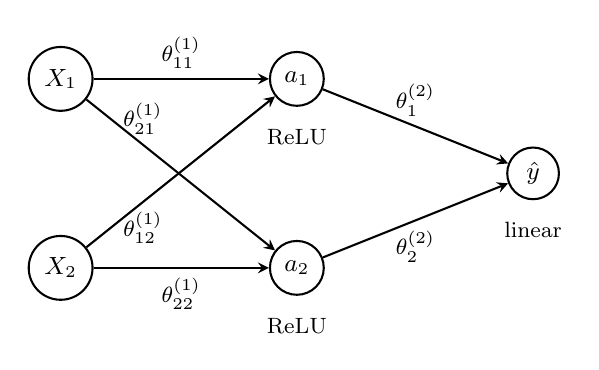
\begin{tikzpicture}[>=stealth, every node/.style={font=\small}]
        \node[circle, draw] (x1) at (0, 1.2)  {$X_1$};
        \node[circle, draw] (x2) at (0, -1.2) {$X_2$};
        \node[circle, draw] (h1) at (3, 1.2)  {$a_1$};
        \node[circle, draw] (h2) at (3, -1.2) {$a_2$};
        \node[circle, draw] (y)  at (6, 0)    {$\hat{y}$};
        \draw[->] (x1) -- node[above, font=\footnotesize]{$\theta^{(1)}_{11}$} (h1);
        \draw[->] (x1) -- node[pos=0.3, above, font=\footnotesize]{$\theta^{(1)}_{21}$} (h2);
        \draw[->] (x2) -- node[pos=0.3, below, font=\footnotesize]{$\theta^{(1)}_{12}$} (h1);
        \draw[->] (x2) -- node[below, font=\footnotesize]{$\theta^{(1)}_{22}$} (h2);
        \draw[->] (h1) -- node[above, font=\footnotesize]{$\theta^{(2)}_{1}$} (y);
        \draw[->] (h2) -- node[below, font=\footnotesize]{$\theta^{(2)}_{2}$} (y);
        \node[below=0.15cm of h1, font=\footnotesize] {ReLU};
        \node[below=0.15cm of h2, font=\footnotesize] {ReLU};
        \node[below=0.15cm of y, font=\footnotesize] {linear};
    \end{tikzpicture}
    \end{center}

    \begin{enumerate}[(a)]
        \item $\theta^{(1)}_{11} = 0.8$ \quad e \quad $\theta^{(1)}_{21} = 0.6$
        \item $\theta^{(1)}_{11} = 0.6$ \quad e \quad $\theta^{(1)}_{21} = 0.6$
        \item $\theta^{(1)}_{11} = 1.0$ \quad e \quad $\theta^{(1)}_{21} = 0.8$
        \item $\theta^{(1)}_{11} = 1.0$ \quad e \quad $\theta^{(1)}_{21} = 0.6$
        \item $\theta^{(1)}_{11} = 1.0$ \quad e \quad $\theta^{(1)}_{21} = 1.0$
        \item $\theta^{(1)}_{11} = 0.6$ \quad e \quad $\theta^{(1)}_{21} = 0.8$
        \item $\theta^{(1)}_{11} = 1.0$ \quad e \quad $\theta^{(1)}_{21} = 0.4$
        \item $\theta^{(1)}_{11} = 0.96$ \quad e \quad $\theta^{(1)}_{21} = 0.6$
    \end{enumerate}
    %d

    \item Um MLP totalmente conectado recebe entradas com $10$ atributos e possui três camadas ocultas com $20$, $20$ e $10$ unidades (todas com ReLU e \textbf{com} viés), seguidas de uma camada de saída com $5$ unidades (também com viés). Qual o número total de parâmetros \emph{treináveis} da rede?
    \begin{enumerate}[(a)]
        \item $1810$
        \item $850$
        \item $900$
        \item $855$
        \item $760$
        \item $925$
        \item $905$
        \item $705$
    \end{enumerate}
    %g

    \item Considere o MLP abaixo, com função de ativação ReLU na camada oculta (1 unidade) e saída linear. As entradas são $X_1 = 1$ e $X_2 = 2$, e a saída esperada é $y = 5$. Os pesos iniciais são $\theta^{(1)}_1 = 1$, $\theta^{(1)}_2 = 1$ e $\theta^{(2)} = 2$ (todos sem viés). A função de custo é $J(\theta) = \tfrac{1}{2}(y - \hat{y})^2$.

    \begin{center}
    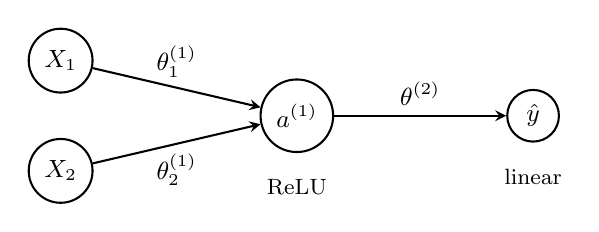
\begin{tikzpicture}[>=stealth, every node/.style={font=\small}]
        \node[circle, draw] (x1) at (0, 0.7) {$X_1$};
        \node[circle, draw] (x2) at (0, -0.7) {$X_2$};
        \node[circle, draw] (h)  at (3, 0)   {$a^{(1)}$};
        \node[circle, draw] (y)  at (6, 0)   {$\hat{y}$};
        \draw[->] (x1) -- node[above]{$\theta^{(1)}_1$} (h);
        \draw[->] (x2) -- node[below]{$\theta^{(1)}_2$} (h);
        \draw[->] (h)  -- node[above]{$\theta^{(2)}$}   (y);
        \node[below=0.2cm of h, font=\footnotesize] {ReLU};
        \node[below=0.2cm of y, font=\footnotesize] {linear};
    \end{tikzpicture}
    \end{center}

    \begin{enumerate}[a)]
        \item Compute o \textit{forward pass} e indique o valor de $\hat{y}$.
        \item Compute o valor da função de custo $J(\theta)$.
        \item Compute os gradientes $\dfrac{\partial J}{\partial \theta^{(2)}}$, $\dfrac{\partial J}{\partial \theta^{(1)}_1}$ e $\dfrac{\partial J}{\partial \theta^{(1)}_2}$.
        \item Realize uma atualização dos três parâmetros usando descida de gradiente estocástica $\theta_{t+1} = \theta_t - \eta \nabla_\theta J$ com taxa de aprendizado $\eta = 0.1$.
    \end{enumerate}

    \item A figura abaixo apresenta seis instâncias de um problema de classificação binária com rótulos $y \in \{-1, +1\}$. A região delimitada pela linha tracejada é a fronteira de decisão de um MLP: tudo que está dentro dela é classificado como $-1$ e tudo que está fora como $+1$.

    \begin{center}
    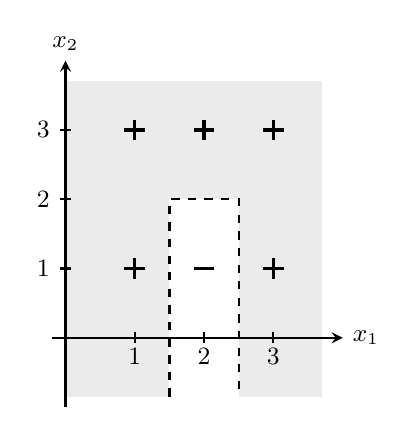
\begin{tikzpicture}[scale=0.88, >=stealth, font=\small]
        % região classificada como +1 (sombreada); a região branca é classificada como -1.
        % Ambas se estendem abaixo de x2 = 0: a faixa negativa não é limitada por baixo.
        \fill[black!8] (0,-0.85) rectangle (3.7,3.7);
        \fill[white] (1.5,-0.85) rectangle (2.5,2);
        \draw[dashed, thick] (1.5,-0.85) -- (1.5,2) -- (2.5,2) -- (2.5,-0.85);
        % eixos
        \draw[->] (-0.2,0) -- (4.0,0) node[right] {$x_1$};
        \draw[->] (0,-1.0) -- (0,4.0) node[above] {$x_2$};
        \foreach \x in {1,2,3} { \draw (\x,0.08) -- (\x,-0.08); \node[below, inner sep=1.5pt, fill=none] at (\x,-0.08) {\x}; }
        \foreach \y in {1,2,3} { \draw (0.08,\y) -- (-0.08,\y) node[left] {\y}; }
        % instâncias positivas
        \foreach \p in {(1,1),(1,3),(2,3),(3,1),(3,3)} {
            \draw[very thick] \p ++(-0.15,0) -- ++(0.30,0);
            \draw[very thick] \p ++(0,-0.15) -- ++(0,0.30);
        }
        % instância negativa
        \draw[very thick] (2,1) ++(-0.15,0) -- ++(0.30,0);
    \end{tikzpicture}
    \end{center}

    \vspace{-0.7em}
    \centerline{\footnotesize As instâncias marcadas com $+$ têm $y = +1$ e a instância marcada com $-$ tem $y = -1$.}
    \centerline{\footnotesize A região sombreada é classificada como $+1$ e a região branca como $-1$.}

    Nas redes abaixo, cada círculo é uma unidade que aplica $\mathrm{sinal}$ à soma ponderada das suas entradas somada ao viés indicado \emph{dentro} do círculo; os números sobre as arestas são os pesos, e as conexões de peso zero foram omitidas. Considere $\mathrm{sinal}(z) = +1$ para $z \geq 0$ e $\mathrm{sinal}(z) = -1$ para $z < 0$. Qual das redes gera exatamente a fronteira de decisão apresentada?

    \begin{center}
    \begin{tabular}{@{}r@{\,}l@{\hspace{0.5em}}r@{\,}l@{\hspace{0.5em}}r@{\,}l@{\hspace{0.5em}}r@{\,}l@{}}
    \textbf{(a)} & \mlpA{1}{1}{-1{,}5}{1}{-1}{2{,}5}{-1}{1} &
    \textbf{(b)} & \mlpB{1}{-1{,}5}{-1}{2{,}5}{1}{-2}{-1}{2} &
    \textbf{(c)} & \mlpA{1}{1}{-1{,}5}{2}{-1}{2}{-1}{1} &
    \textbf{(d)} & \mlpB{1}{-1{,}5}{-1}{2{,}5}{-1}{2}{1}{-2} \\[4em]
    \textbf{(e)} & \mlpA{1}{-1}{2{,}5}{2}{-1}{2}{-1}{1} &
    \textbf{(f)} & \mlpB{1}{-1{,}5}{-1}{2{,}5}{-1}{2}{-1}{2} &
    \textbf{(g)} & \mlpA{1}{1}{-1{,}5}{1}{-1}{2{,}5}{1}{-1} &
    \textbf{(h)} & \mlpB{1}{-1{,}5}{-1}{2{,}5}{-1}{2}{-1}{4} \\
    \end{tabular}
    \end{center}
    %f

    \item Considere um MLP vetorizado com $\mathbf{Z}^{(l)} = \mathbf{A}^{(l-1)}{\mathbf{\Theta}^{(l)}}^{\top} + \mathbf{b}^{(l)}$, ReLU na camada oculta e sigmoide na camada de saída. Para o minilote de duas instâncias
    \[
    \mathbf{X} = \begin{bmatrix} 1 & 2 \\ 2 & 0 \end{bmatrix}, \quad
    \mathbf{\Theta}^{(1)} = \begin{bmatrix} 1 & -1 \\ 0 & 2 \end{bmatrix}, \quad
    \mathbf{b}^{(1)} = \begin{bmatrix} 0 & -1 \end{bmatrix}, \quad
    \mathbf{\Theta}^{(2)} = \begin{bmatrix} 1 & 2 \end{bmatrix}, \quad
    b^{(2)} = -2 ,
    \]
    e sabendo que $\sigma(0) = 0{,}500$, $\sigma(2) \approx 0{,}881$, $\sigma(3) \approx 0{,}953$, $\sigma(4) \approx 0{,}982$ e $\sigma(6) \approx 0{,}998$, qual é o vetor de saídas $\hat{\mathbf{y}}$ do minilote?

    \begin{enumerate}[(a)]
        \item $\hat{\mathbf{y}} = (0{,}953;\ 0{,}119)$
        \item $\hat{\mathbf{y}} = (0{,}998;\ 0{,}881)$
        \item $\hat{\mathbf{y}} = (0{,}500;\ 0{,}982)$
        \item $\hat{\mathbf{y}} = (0{,}982;\ 0{,}500)$
        \item $\hat{\mathbf{y}} = (0{,}953;\ 0{,}500)$
        \item $\hat{\mathbf{y}} = (0{,}998;\ 0{,}500)$
        \item $\hat{\mathbf{y}} = (0{,}982;\ 0{,}982)$
        \item $\hat{\mathbf{y}} = (0{,}119;\ 0{,}953)$
    \end{enumerate}
    %d

    \item Considere o MLP abaixo, com duas unidades ReLU na camada oculta e saída linear. A entrada é $x = 2$ e a saída esperada é $y = 3$. A função de custo é $J = \tfrac{1}{2}(y - \hat{y})^2$ e os parâmetros são
    \[
    \mathbf{\Theta}^{(1)} = \begin{bmatrix} 0{,}5 \\ -1 \end{bmatrix}, \quad
    \mathbf{b}^{(1)} = \begin{bmatrix} 1 & 0{,}5 \end{bmatrix}, \quad
    \mathbf{\Theta}^{(2)} = \begin{bmatrix} 1{,}5 & 2 \end{bmatrix}, \quad
    b^{(2)} = -0{,}5 .
    \]

    \begin{center}
    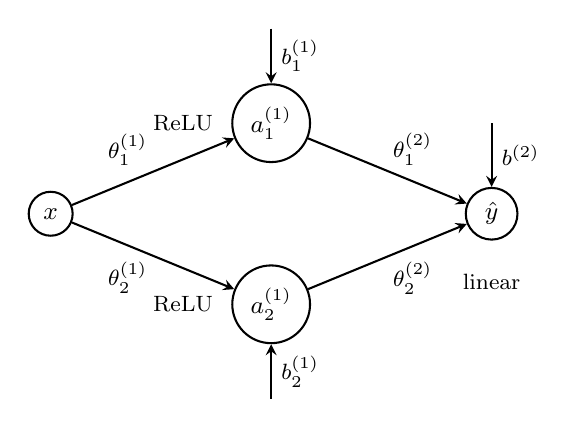
\begin{tikzpicture}[>=stealth, every node/.style={font=\small}]
        \node[circle, draw] (x)  at (0, 0)      {$x$};
        \node[circle, draw] (h1) at (2.8, 1.15)  {$a^{(1)}_1$};
        \node[circle, draw] (h2) at (2.8, -1.15) {$a^{(1)}_2$};
        \node[circle, draw] (y)  at (5.6, 0)    {$\hat{y}$};
        % pesos
        \draw[->] (x)  -- node[above left=-0.08cm, font=\footnotesize]{$\theta^{(1)}_1$} (h1);
        \draw[->] (x)  -- node[below left=-0.08cm, font=\footnotesize]{$\theta^{(1)}_2$} (h2);
        \draw[->] (h1) -- node[above right=-0.08cm, font=\footnotesize]{$\theta^{(2)}_1$} (y);
        \draw[->] (h2) -- node[below right=-0.08cm, font=\footnotesize]{$\theta^{(2)}_2$} (y);
        % vieses como arestas que chegam nas unidades
        \draw[->] (2.8, 2.35)  -- node[right, font=\footnotesize]{$b^{(1)}_1$} (h1);
        \draw[->] (2.8, -2.35) -- node[right, font=\footnotesize]{$b^{(1)}_2$} (h2);
        \draw[->] (5.6, 1.15)  -- node[right, font=\footnotesize]{$b^{(2)}$}   (y);
        % funções de ativação, junto de cada unidade
        \node[left=0.10cm of h1, font=\footnotesize] {ReLU};
        \node[left=0.10cm of h2, font=\footnotesize] {ReLU};
        \node[below=0.30cm of y, font=\footnotesize] {linear};
    \end{tikzpicture}
    \end{center}

    Qual o valor de $\dfrac{\partial J}{\partial b^{(1)}_1}$?

    \begin{enumerate}[(a)]
        \item $0$
        \item $-0{,}25$
        \item $-0{,}50$
        \item $+0{,}75$
        \item $-0{,}75$
        \item $-1{,}00$
        \item $-1{,}25$
        \item $-1{,}50$
    \end{enumerate}
    %e

    \item Considere o MLP da figura abaixo, com uma entrada $x$, três unidades ocultas com ativação $\mathrm{a}[z] = \mathrm{ReLU}[z] = \max(0, z)$ e uma saída linear
    \[
    y = \phi_0 + \phi_1 h_1 + \phi_2 h_2 + \phi_3 h_3, \qquad h_k = \mathrm{a}[\theta_{k0} + \theta_{k1} x],
    \]
    com $\phi_0 = 0{,}2$. Os gráficos mostram, para $x \in [0, 2]$, as pré-ativações, as ativações, as ativações ponderadas pelos pesos da camada de saída e o viés $\phi_0$ da saída.

    \begin{center}
    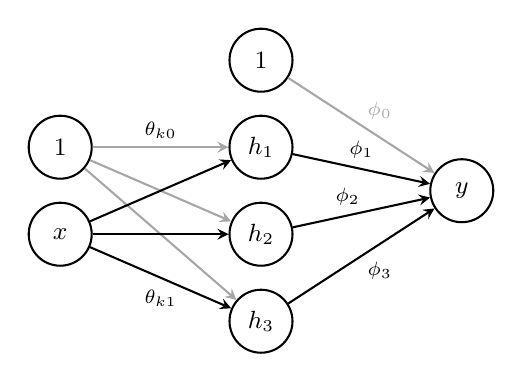
\begin{tikzpicture}[>=stealth, scale=0.85, every node/.style={font=\small}]
        \node[circle, draw, minimum size=8mm] (one) at (0, 1.3) {$1$};
        \node[circle, draw, minimum size=8mm] (x)   at (0, 0)   {$x$};
        \node[circle, draw, minimum size=8mm] (h1)  at (3, 1.3)  {$h_1$};
        \node[circle, draw, minimum size=8mm] (h2)  at (3, 0)    {$h_2$};
        \node[circle, draw, minimum size=8mm] (h3)  at (3, -1.3) {$h_3$};
        \node[circle, draw, minimum size=8mm] (one2) at (3, 2.6) {$1$};
        \node[circle, draw, minimum size=8mm] (y)   at (6, 0.65)   {$y$};
        \draw[->, gray!70] (one) -- (h1); \draw[->, gray!70] (one) -- (h2); \draw[->, gray!70] (one) -- (h3);
        \draw[->] (x) -- (h1); \draw[->] (x) -- (h2); \draw[->] (x) -- (h3);
        \node[font=\scriptsize] at (1.5, 1.55) {$\theta_{k0}$};
        \node[font=\scriptsize] at (1.5, -0.95) {$\theta_{k1}$};
        \draw[->, gray!70] (one2) -- node[above right=-2pt, font=\scriptsize]{$\phi_0$} (y);
        \draw[->] (h1) -- node[above, font=\scriptsize]{$\phi_1$} (y);
        \draw[->] (h2) -- node[above, font=\scriptsize, pos=0.4]{$\phi_2$} (y);
        \draw[->] (h3) -- node[below right=-2pt, font=\scriptsize]{$\phi_3$} (y);
    \end{tikzpicture}

    \vspace{0.4em}
    \setlength{\tabcolsep}{4pt}
    \begin{tabular}{cccc}
    \fpA{(0,0.6) -- (2,-0.4)}{$\theta_{10} + \theta_{11}x$} &
    \fpA{(0,-0.2) -- (2,0.8)}{$\theta_{20} + \theta_{21}x$} &
    \fpA{(0,-0.8) -- (2,0.2)}{$\theta_{30} + \theta_{31}x$} & \\[0.5em]
    \fpA{(0,0.6) -- (1.2,0) -- (2,0)}{$h_1$} &
    \fpA{(0,0) -- (0.4,0) -- (2,0.8)}{$h_2$} &
    \fpA{(0,0) -- (1.6,0) -- (2,0.2)}{$h_3$} & \\[0.5em]
    \fpA{(0,0.6) -- (1.2,0) -- (2,0)}{$\phi_1 h_1$} &
    \fpA{(0,0) -- (0.4,0) -- (2,-0.8)}{$\phi_2 h_2$} &
    \fpA{(0,0) -- (1.6,0) -- (2,0.6)}{$\phi_3 h_3$} &
    \fpA{(0,0.2) -- (2,0.2)}{$\phi_0$} \\
    \end{tabular}
    \end{center}

    Qual dos gráficos abaixo representa a saída $y$ desse MLP para $x \in [0, 2]$?

    \begin{center}
    \setlength{\tabcolsep}{1pt}
    \scalebox{0.93}{%
    \begin{tabular}{r@{\,}lr@{\,}lr@{\,}lr@{\,}l}
    \textbf{(a)} & \fpB{(0,0.6) -- (0.4,0.4) -- (1.2,-0.4) -- (1.6,-0.6) -- (2,-0.2)} &
    \textbf{(b)} & \fpB{(0,0.6) -- (0.4,0.4) -- (1.2,0.4) -- (1.6,0.6) -- (2,1.0)} &
    \textbf{(c)} & \fpB{(0,0.8) -- (0.4,0.6) -- (1.2,-0.2) -- (1.6,-0.4) -- (2,0)} &
    \textbf{(d)} & \fpB{(0,-1.4) -- (2,-0.4)} \\[1.4em]
    \textbf{(e)} & \fpB{(0,0.6) -- (0.4,0.6) -- (1.2,0.2) -- (1.6,0.2) -- (2,0.8)} &
    \textbf{(f)} & \fpB{(0,0.8) -- (0.4,0.6) -- (1.2,0.6) -- (1.6,0.8) -- (2,1.2)} &
    \textbf{(g)} & \fpB{(0,0.8) -- (0.4,0.6) -- (1.2,-0.2) -- (1.6,-0.4) -- (2,-0.6)} &
    \textbf{(h)} & \fpB{(0,0.2) -- (0.4,0.2) -- (1.2,-0.2) -- (1.6,-0.2) -- (2,0.4)} \\
    \end{tabular}
    }
    \end{center}
    %c

    \item Considere o MLP abaixo, com duas unidades ReLU na camada oculta e uma unidade sigmoide na saída, treinado com a entropia cruzada binária $J = -\bigl(y\ln\hat{y} + (1-y)\ln(1-\hat{y})\bigr)$. A entrada é $x = 2$, o rótulo é $y = 1$ e os parâmetros são
    \[
    \mathbf{\Theta}^{(1)} = \begin{bmatrix} 1 \\ -0{,}5 \end{bmatrix}, \quad
    \mathbf{b}^{(1)} = \begin{bmatrix} -1 & 2 \end{bmatrix}, \quad
    \mathbf{\Theta}^{(2)} = \begin{bmatrix} 2 & -1{,}5 \end{bmatrix}, \quad
    b^{(2)} = -0{,}5 .
    \]

    \begin{center}
    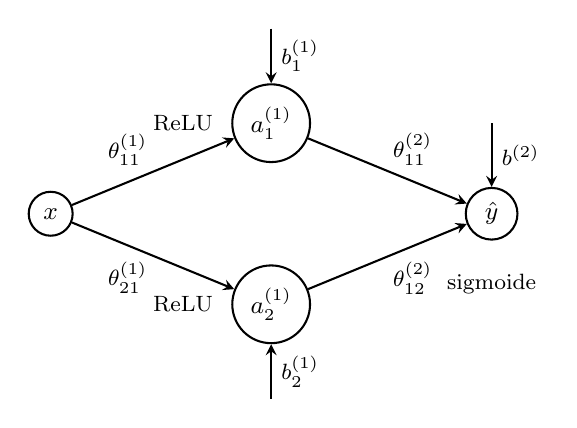
\begin{tikzpicture}[>=stealth, every node/.style={font=\small}]
        \node[circle, draw] (x)  at (0, 0)      {$x$};
        \node[circle, draw] (h1) at (2.8, 1.15)  {$a^{(1)}_1$};
        \node[circle, draw] (h2) at (2.8, -1.15) {$a^{(1)}_2$};
        \node[circle, draw] (y)  at (5.6, 0)    {$\hat{y}$};
        \draw[->] (x)  -- node[above left=-0.08cm, font=\footnotesize]{$\theta^{(1)}_{11}$} (h1);
        \draw[->] (x)  -- node[below left=-0.08cm, font=\footnotesize]{$\theta^{(1)}_{21}$} (h2);
        \draw[->] (h1) -- node[above right=-0.08cm, font=\footnotesize]{$\theta^{(2)}_{11}$} (y);
        \draw[->] (h2) -- node[below right=-0.08cm, font=\footnotesize]{$\theta^{(2)}_{12}$} (y);
        \draw[->] (2.8, 2.35)  -- node[right, font=\footnotesize]{$b^{(1)}_1$} (h1);
        \draw[->] (2.8, -2.35) -- node[right, font=\footnotesize]{$b^{(1)}_2$} (h2);
        \draw[->] (5.6, 1.15)  -- node[right, font=\footnotesize]{$b^{(2)}$}   (y);
        \node[left=0.10cm of h1, font=\footnotesize] {ReLU};
        \node[left=0.10cm of h2, font=\footnotesize] {ReLU};
        \node[below=0.30cm of y, font=\footnotesize] {sigmoide};
    \end{tikzpicture}
    \end{center}

    Sabendo que $\sigma(0) = 0{,}5$ e que a derivada da entropia cruzada binária em relação à saída é
    \[
    \frac{\partial J}{\partial \hat{y}} = -\frac{y}{\hat{y}} + \frac{1 - y}{1 - \hat{y}},
    \]
    qual o valor de $\dfrac{\partial J}{\partial \theta^{(1)}_{21}}$?

    \begin{enumerate}[(a)]
        \item $+0{,}75$
        \item $-1{,}0$
        \item $-1{,}5$
        \item $+0{,}375$
        \item $+1{,}5$
        \item $+6{,}0$
        \item $-2{,}0$
        \item $-0{,}375$
    \end{enumerate}
    %e

\end{enumerate}

\newpage

\subsection*{Gabarito}
\color{blue}
\begin{enumerate}[1)]

    \item a. Cada unidade computa o produto escalar entre o vetor de entradas e o vetor de pesos (somado ao bias) para formar a pré-ativação; a função de ativação é aplicada depois, sobre esse resultado. \textit{Backpropagation} e descida de gradiente pertencem ao treinamento, não ao \textit{forward pass}.

    \item b. O \textit{forward pass} computa as saídas de cada unidade até produzir a predição, e o \textit{backward pass} computa os gradientes da função de custo em relação aos pesos. As alternativas (d) e (e) confundem as duas fases com os algoritmos que as utilizam.

    \item $3D + 1 + (K - 1)D(D + 1)$. Repare que essa expressão não é a única resposta possível para o exercício. Dependendo de como você desenvolver a questão poderá chegar em expressões equivalentes como por exemplo: $2D + (K - 1)DD + KD + 1$. Contagem por partes: da entrada para a primeira camada oculta são $D$ pesos e $D$ bias; entre camadas ocultas são $(K-1)$ transições com $D^2$ pesos e $D$ bias cada; da última camada oculta para a saída são $D$ pesos e $1$ bias. Somando: $2D + (K-1)D(D+1) + D + 1 = 3D + 1 + (K-1)D(D+1)$

    \item \textit{Forward Pass}: onde as saídas são calculadas; \textit{Loss Function}: onde a diferença entre a saída e o valor esperado são comparadas; \textit{Backward Pass}: onde os gradientes da função de custo em relação a cada um dos pesos é calculado; \textit{Optimizer}: onde os pesos são atualizados.

    \item Considerando ReLU $\varphi(z)=\max(0,z)$ em todas as unidades (inclusive na saída) e taxa de aprendizado $\eta = 0.1$.

    \textit{Forward Pass:}
    \begin{align*}
        \mathbf{z}^{(1)} &= \mathbf{\Theta}^{(1)}\mathbf{X} + \boldsymbol{\beta}^{(1)} = \begin{bmatrix}0.5 & -0.2\\ 0.1 & 0.2\end{bmatrix}\begin{bmatrix}2\\ 1\end{bmatrix} + \begin{bmatrix}0.2\\ -0.1\end{bmatrix} = \begin{bmatrix}1.0\\ 0.3\end{bmatrix}, \quad \mathbf{a}^{(1)}=\varphi(\mathbf{z}^{(1)})=\begin{bmatrix}1.0\\ 0.3\end{bmatrix}\\
        z^{(2)} &= \mathbf{\Theta}^{(2)}\mathbf{a}^{(1)} + \beta^{(2)} = \begin{bmatrix}0.2 & -0.1\end{bmatrix}\begin{bmatrix}1.0\\ 0.3\end{bmatrix} + 0.4 = 0.57, \quad \hat{y}=a^{(2)}=\varphi(0.57)=0.57
    \end{align*}

    \textit{Loss:} $J=(\hat{y}-y)^2 = (0.57-1)^2 = 0.1849$.

    \textit{Backward Pass:} como $\frac{\partial J}{\partial \hat{y}}=2(\hat{y}-y)=-0.86$ e $\varphi'(z)=1$ para $z>0$,
    \begin{align*}
        \delta^{(2)} &= 2(\hat{y}-y)\odot\varphi'(z^{(2)}) = -0.86\\
        \frac{\partial J}{\partial \mathbf{\Theta}^{(2)}} &= \delta^{(2)}\mathbf{a}^{(1)\top} = \begin{bmatrix}-0.86 & -0.258\end{bmatrix}, \quad \frac{\partial J}{\partial \beta^{(2)}} = \delta^{(2)} = -0.86\\
        \boldsymbol{\delta}^{(1)} &= (\delta^{(2)}\mathbf{\Theta}^{(2)})\odot\varphi'(\mathbf{z}^{(1)}) = \begin{bmatrix}-0.172 & 0.086\end{bmatrix}\\
        \frac{\partial J}{\partial \mathbf{\Theta}^{(1)}} &= \boldsymbol{\delta}^{(1)\top}\mathbf{X}^\top = \begin{bmatrix}-0.172\\ 0.086\end{bmatrix}\begin{bmatrix}2 & 1\end{bmatrix} = \begin{bmatrix}-0.344 & -0.172\\ 0.172 & 0.086\end{bmatrix}, \quad \frac{\partial J}{\partial \boldsymbol{\beta}^{(1)}} = \boldsymbol{\delta}^{(1)} = \begin{bmatrix}-0.172 & 0.086\end{bmatrix}
    \end{align*}

    \textit{Atualização (SGD, $\theta_{t+1}=\theta_t-\eta\nabla J$):}
    \begin{align*}
        \mathbf{\Theta}^{(1)} &\leftarrow \begin{bmatrix}0.5 & -0.2\\ 0.1 & 0.2\end{bmatrix} - 0.1\begin{bmatrix}-0.344 & -0.172\\ 0.172 & 0.086\end{bmatrix} = \begin{bmatrix}0.5344 & -0.1828\\ 0.0828 & 0.1914\end{bmatrix}\\
        \boldsymbol{\beta}^{(1)} &\leftarrow \begin{bmatrix}0.2 & -0.1\end{bmatrix} - 0.1\begin{bmatrix}-0.172 & 0.086\end{bmatrix} = \begin{bmatrix}0.2172 & -0.1086\end{bmatrix}\\
        \mathbf{\Theta}^{(2)} &\leftarrow \begin{bmatrix}0.2 & -0.1\end{bmatrix} - 0.1\begin{bmatrix}-0.86 & -0.258\end{bmatrix} = \begin{bmatrix}0.286 & -0.0742\end{bmatrix}\\
        \beta^{(2)} &\leftarrow 0.4 - 0.1(-0.86) = 0.486
    \end{align*}

    \item d. \textit{Forward pass}:
    \begin{align*}
        z_1 &= X_1\,\theta^{(1)}_{11} + X_2\,\theta^{(1)}_{12} = 1\cdot 1 + 2\cdot(-1) = -1 \;\Rightarrow\; a_1 = \mathrm{ReLU}(-1) = 0 \\
        z_2 &= X_1\,\theta^{(1)}_{21} + X_2\,\theta^{(1)}_{22} = 1\cdot 1 + 2\cdot 1 = 3 \;\Rightarrow\; a_2 = \mathrm{ReLU}(3) = 3 \\
        \hat{y} &= a_1\,\theta^{(2)}_{1} + a_2\,\theta^{(2)}_{2} = 0\cdot 1 + 3\cdot 2 = 6
    \end{align*}
    $\partial J/\partial \hat{y} = \hat{y} - y = 6 - 4 = 2$. Os gradientes pedidos:
    \begin{align*}
        \frac{\partial J}{\partial \theta^{(1)}_{11}} &= \underbrace{(\hat{y}-y)}_{2}\cdot \underbrace{\theta^{(2)}_{1}}_{1}\cdot \underbrace{\mathrm{ReLU}'(z_1)}_{0}\cdot \underbrace{X_1}_{1} = 0 \quad (\text{unidade } a_1 \text{ inativa}) \\
        \frac{\partial J}{\partial \theta^{(1)}_{21}} &= \underbrace{(\hat{y}-y)}_{2}\cdot \underbrace{\theta^{(2)}_{2}}_{2}\cdot \underbrace{\mathrm{ReLU}'(z_2)}_{1}\cdot \underbrace{X_1}_{1} = 4
    \end{align*}
    Atualização com $\eta = 0.1$: $\theta^{(1)}_{11} \leftarrow 1 - 0.1\cdot 0 = 1.0$ e $\theta^{(1)}_{21} \leftarrow 1 - 0.1\cdot 4 = 0.6$. O ponto-chave é que $a_1$ recebe pré-ativação negativa, logo $\mathrm{ReLU}' = 0$ e $\theta^{(1)}_{11}$ \emph{não é atualizado}. As alternativas (a), (b) e (f) tratam $a_1$ como ativa (atualizam $\theta^{(1)}_{11}$), ignorando $\mathrm{ReLU}'(-1) = 0$; (c) usa gradiente $2$ para $\theta^{(1)}_{21}$ (esquece o fator $\theta^{(2)}_2 = 2$), obtendo $1 - 0.1\cdot 2 = 0.8$; (g) usa gradiente $6$ ($1 - 0.1\cdot 6 = 0.4$); (e) não atualiza $\theta^{(1)}_{21}$; (h) aplica uma pequena atualização espúria a $\theta^{(1)}_{11}$.

    \item g. Cada camada totalmente conectada tem $n_{\text{in}}\cdot n_{\text{out}} + n_{\text{out}}$ parâmetros (pesos mais vieses): entrada $\to h_1$: $10\cdot 20 + 20 = 220$; $h_1 \to h_2$: $20\cdot 20 + 20 = 420$; $h_2 \to h_3$: $20\cdot 10 + 10 = 210$; $h_3 \to$ saída: $10\cdot 5 + 5 = 55$. Total: $220 + 420 + 210 + 55 = 905$. A alternativa (b) $850$ ignora todos os vieses; (c) $900$ esquece o viés da camada de saída ($850 + 50$); (d) $855$ é um erro aritmético; (a) $1810$ dobra a contagem; (e), (f) e (h) são outros erros de contagem.

    \item Dados: $X_1 = 1$, $X_2 = 2$, $y = 5$, $\theta^{(1)}_1 = 1$, $\theta^{(1)}_2 = 1$, $\theta^{(2)} = 2$, $\eta = 0.1$.
    \begin{enumerate}[a)]
        \item \textit{Forward pass}:
        \begin{align*}
            z^{(1)} &= X_1 \cdot \theta^{(1)}_1 + X_2 \cdot \theta^{(1)}_2 = 1 \cdot 1 + 2 \cdot 1 = 3 \\
            a^{(1)} &= \mathrm{ReLU}(z^{(1)}) = \max(0, 3) = 3 \\
            z^{(2)} &= a^{(1)} \cdot \theta^{(2)} = 3 \cdot 2 = 6 \\
            \hat{y} &= z^{(2)} = 6 \quad \text{(saída linear)}
        \end{align*}
        \item \textit{Função de custo}: $J(\theta) = \tfrac{1}{2}(y - \hat{y})^2 = \tfrac{1}{2}(5 - 6)^2 = 0.5$.
        \item \textit{Backward pass} (regra da cadeia):
        \begin{align*}
            \frac{\partial J}{\partial \hat{y}} &= -(y - \hat{y}) = -(5 - 6) = 1 \\
            \frac{\partial J}{\partial \theta^{(2)}} &= \frac{\partial J}{\partial \hat{y}} \cdot a^{(1)} = 1 \cdot 3 = 3 \\
            \frac{\partial J}{\partial a^{(1)}} &= \frac{\partial J}{\partial \hat{y}} \cdot \theta^{(2)} = 1 \cdot 2 = 2 \\
            \frac{\partial a^{(1)}}{\partial z^{(1)}} &= \mathrm{ReLU}'(z^{(1)}) = 1 \quad (\text{pois } z^{(1)} = 3 > 0) \\
            \frac{\partial J}{\partial z^{(1)}} &= \frac{\partial J}{\partial a^{(1)}} \cdot \frac{\partial a^{(1)}}{\partial z^{(1)}} = 2 \cdot 1 = 2 \\
            \frac{\partial J}{\partial \theta^{(1)}_1} &= \frac{\partial J}{\partial z^{(1)}} \cdot X_1 = 2 \cdot 1 = 2 \\
            \frac{\partial J}{\partial \theta^{(1)}_2} &= \frac{\partial J}{\partial z^{(1)}} \cdot X_2 = 2 \cdot 2 = 4
        \end{align*}
        \item \textit{Atualização SGD} com $\eta = 0.1$:
        \begin{align*}
            \theta^{(2)}_{t+1}      &= 2 - 0.1 \cdot 3 = 1.7 \\
            \theta^{(1)}_{1,\,t+1}  &= 1 - 0.1 \cdot 2 = 0.8 \\
            \theta^{(1)}_{2,\,t+1}  &= 1 - 0.1 \cdot 4 = 0.6
        \end{align*}
    \end{enumerate}

    \item f. \textbf{Contagem de unidades.} A região negativa é a interseção de \emph{três} semiplanos: $x_1 > 1{,}5$, $x_1 < 2{,}5$ e $x_2 < 2$. Cada semiplano exige uma unidade oculta, e é preciso mais uma unidade na saída para combiná-los com um E lógico, totalizando \textbf{quatro} unidades. As redes de três unidades têm apenas duas ocultas e só conseguem representar a interseção de dois semiplanos, que é sempre uma região ilimitada; nenhuma delas isola a instância $(2;1)$ sem arrastar junto outra instância positiva. Isso elimina de imediato as alternativas (a), (c), (e) e (g), restando apenas quatro candidatas. \textbf{Verificação da alternativa (f).} As três unidades ocultas calculam $h_1 = \mathrm{sinal}(x_1 - 1{,}5)$, $h_2 = \mathrm{sinal}(2{,}5 - x_1)$ e $h_3 = \mathrm{sinal}(2 - x_2)$, e a saída calcula $\hat{y} = \mathrm{sinal}(2 - h_1 - h_2 - h_3)$. Como $h_1 + h_2 + h_3 \in \{3, 1, -1, -3\}$, a saída vale $-1$ apenas quando a soma é $3$, isto é, quando as três condições valem ao mesmo tempo. Conferindo: $(2;1)$ dá $h = (+1, +1, +1)$ e soma $3$, logo $\hat{y} = \mathrm{sinal}(-1) = -1$; $(1;1)$ e $(3;1)$ dão soma $1$ (falha um dos limiares em $x_1$) e $(1;3)$, $(2;3)$, $(3;3)$ dão soma $1$ ou $-1$ (falha o limiar em $x_2$), todas com $\hat{y} = +1$. Quanto às demais: (a) tem três unidades e nem sequer conecta $x_2$, as duas ocultas recortam a faixa vertical inteira $1{,}5 < x_1 < 2{,}5$ e classificam $(2;3)$ como $-1$; (b) tem quatro unidades, mas a terceira oculta usa peso $+1$ e viés $-2$, recortando $x_2 > 2$ em vez de $x_2 < 2$, e erra $(2;1)$ e $(2;3)$; (c) tem três unidades e define o quadrante $x_1 > 1{,}5$ e $x_2 < 2$, ilimitado à direita, classificando $(3;1)$ como $-1$; (d) tem as ocultas corretas, mas os pesos de saída são $+1$ e o viés é $-2$, o que inverte a decisão (prediz $+1$ dentro da região e $-1$ fora) e erra as seis instâncias; (e) tem três unidades e define o quadrante $x_1 < 2{,}5$ e $x_2 < 2$, ilimitado à esquerda, classificando $(1;1)$ como $-1$; (g) tem três unidades, ignora $x_2$ e ainda inverte a saída com pesos $+1$ e viés $-1$, errando cinco das seis instâncias; (h) tem as ocultas corretas, mas o viés da saída é $4$: como $\mathrm{sinal}(4 - 3) = +1$, a rede nunca prediz $-1$ e erra $(2;1)$.

    \item d.
    \[
    \mathbf{Z}^{(1)} = \mathbf{X}\,{\mathbf{\Theta}^{(1)}}^{\top} + \mathbf{b}^{(1)}
    = \begin{bmatrix} 1 & 2 \\ 2 & 0 \end{bmatrix}\begin{bmatrix} 1 & 0 \\ -1 & 2 \end{bmatrix} + \begin{bmatrix} 0 & -1 \end{bmatrix}
    = \begin{bmatrix} -1 & 4 \\ 2 & 0 \end{bmatrix} + \begin{bmatrix} 0 & -1 \end{bmatrix}
    = \begin{bmatrix} -1 & 3 \\ 2 & -1 \end{bmatrix},
    \]
    \[
    \mathbf{A}^{(1)} = \mathrm{ReLU}\bigl(\mathbf{Z}^{(1)}\bigr) = \begin{bmatrix} 0 & 3 \\ 2 & 0 \end{bmatrix},
    \qquad
    \mathbf{Z}^{(2)} = \mathbf{A}^{(1)}{\mathbf{\Theta}^{(2)}}^{\top} + b^{(2)} = \begin{bmatrix} 6 \\ 2 \end{bmatrix} - 2 = \begin{bmatrix} 4 \\ 0 \end{bmatrix},
    \]
    \[
    \hat{\mathbf{y}} = \sigma\bigl(\mathbf{Z}^{(2)}\bigr) = (0{,}982;\ 0{,}500).
    \]
    Em (a), a ReLU foi omitida e $\mathbf{Z}^{(1)}$ propagado direto, chegando a $\mathbf{Z}^{(2)} = (3; -2)$; em (b), o viés $b^{(2)} = -2$ foi esquecido, chegando a $\mathbf{Z}^{(2)} = (6; 2)$; em (c), a ordem das duas instâncias do minilote foi invertida; em (e), $\mathbf{\Theta}^{(1)}$ foi usado sem transpor, chegando a $\mathbf{Z}^{(2)} = (3; 0)$; em (f), o viés $\mathbf{b}^{(1)}$ foi esquecido, o que deixa $\mathbf{A}^{(1)} = [\,0\ \ 4\,;\ 2\ \ 0\,]$ e $\mathbf{Z}^{(2)} = (6; 0)$; em (g), a saída da primeira instância foi repetida nas duas linhas; (h) combina o erro de (a), omitir a ReLU, com a inversão das instâncias de (c).

    \item e. \textit{Forward pass:}
    \[
    \mathbf{z}^{(1)} = x\,{\mathbf{\Theta}^{(1)}}^{\top} + \mathbf{b}^{(1)}
    = \begin{bmatrix} 0{,}5 \cdot 2 + 1 & -1 \cdot 2 + 0{,}5 \end{bmatrix} = \begin{bmatrix} 2 & -1{,}5 \end{bmatrix},
    \qquad
    \mathbf{a}^{(1)} = \mathrm{ReLU}(\mathbf{z}^{(1)}) = \begin{bmatrix} 2 & 0 \end{bmatrix},
    \]
    \[
    z^{(2)} = 1{,}5 \cdot 2 + 2 \cdot 0 - 0{,}5 = 2{,}5, \qquad \hat{y} = 2{,}5, \qquad J = \tfrac{1}{2}(3 - 2{,}5)^2 = 0{,}125 .
    \]
    \textit{Backward pass:} com saída linear, $\dfrac{\partial J}{\partial z^{(2)}} = \hat{y} - y = -0{,}5$. Propagando para a primeira unidade oculta,
    \[
    \frac{\partial J}{\partial a^{(1)}_1} = -0{,}5 \cdot \theta^{(2)}_1 = -0{,}5 \cdot 1{,}5 = -0{,}75,
    \qquad
    \frac{\partial J}{\partial z^{(1)}_1} = -0{,}75 \cdot \mathrm{ReLU}'(2) = -0{,}75 .
    \]
    Como $z^{(1)}_1 = \theta^{(1)}_1 x + b^{(1)}_1$, temos $\partial z^{(1)}_1 / \partial b^{(1)}_1 = 1$ e portanto $\partial J / \partial b^{(1)}_1 = -0{,}75$. A alternativa (a) é o gradiente da \emph{segunda} unidade, que está morta ($z^{(1)}_2 = -1{,}5 < 0$, logo $\mathrm{ReLU}' = 0$); (b) deriva $\tfrac{1}{2}(y - \hat{y})^2$ mantendo o fator $\tfrac{1}{2}$ na derivada; (c) para em $\partial J / \partial z^{(2)}$ e não multiplica pelo peso $\theta^{(2)}_1$; (d) usa $y - \hat{y}$ em vez de $\hat{y} - y$, invertendo o sinal do gradiente; (f) usa $\theta^{(2)}_2 = 2$ no lugar de $\theta^{(2)}_1 = 1{,}5$; (g) soma indevidamente os gradientes dos dois caminhos, $-0{,}75$ e $-0{,}5$; (h) trata o viés como um peso e multiplica o gradiente pela entrada $x = 2$.

    \item c. Lendo os gráficos: $h_1 = \mathrm{ReLU}[0{,}6 - 0{,}5x]$ (ativa para $x < 1{,}2$), $h_2 = \mathrm{ReLU}[-0{,}2 + 0{,}5x]$ (ativa para $x > 0{,}4$) e $h_3 = \mathrm{ReLU}[-0{,}8 + 0{,}5x]$ (ativa para $x > 1{,}6$), com $\phi_1 = 1$, $\phi_2 = -1$ e $\phi_3 = 3$. Somando as três ativações ponderadas e $\phi_0 = 0{,}2$, as dobras ficam em $x = 0{,}4$, $1{,}2$ e $1{,}6$:
    \[
    \begin{array}{c|ccccc}
    x & 0 & 0{,}4 & 1{,}2 & 1{,}6 & 2 \\\hline
    \phi_1 h_1 & 0{,}6 & 0{,}4 & 0 & 0 & 0 \\
    \phi_2 h_2 & 0 & 0 & -0{,}4 & -0{,}6 & -0{,}8 \\
    \phi_3 h_3 & 0 & 0 & 0 & 0 & 0{,}6 \\\hline
    y & 0{,}8 & 0{,}6 & -0{,}2 & -0{,}4 & 0
    \end{array}
    \]
    A saída é linear por partes, com inclinações $-0{,}5$, $-1$, $-0{,}5$ e $+1$, o que corresponde ao gráfico (c). Em (a), o viés $\phi_0$ foi esquecido e a curva fica deslocada $0{,}2$ para baixo; (b) combina dois erros, esquece o viés $\phi_0$ e soma as ativações $h_k$ sem ponderá-las por $\phi_k$; em (d), somaram-se as pré-ativações em vez das ativações, e sem a ReLU a rede colapsa em uma reta, $y = -1{,}4 + 0{,}5x$; em (e), $h_2$ foi ativada no lado errado da dobra, como se a unidade valesse $\mathrm{ReLU}[0{,}2 - 0{,}5x]$; em (f), as ativações $h_k$ foram somadas sem ponderação por $\phi_k$; em (g), a contribuição de $h_3$ foi ignorada e a descida continua após $x = 1{,}6$; em (h), $h_1$ foi ativada no lado errado da dobra, como se a unidade valesse $\mathrm{ReLU}[-0{,}6 + 0{,}5x]$.

    \item e. \textit{Forward:} $\mathbf{z}^{(1)} = x\,{\mathbf{\Theta}^{(1)}}^{\top} + \mathbf{b}^{(1)} = 2\begin{bmatrix} 1 & -0{,}5 \end{bmatrix} + \begin{bmatrix} -1 & 2 \end{bmatrix} = \begin{bmatrix} 1 & 1 \end{bmatrix}$, $\mathbf{a}^{(1)} = \begin{bmatrix} 1 & 1 \end{bmatrix}$, $z^{(2)} = \mathbf{a}^{(1)}{\mathbf{\Theta}^{(2)}}^{\top} + b^{(2)} = 2 - 1{,}5 - 0{,}5 = 0$ e $\hat{y} = \sigma(0) = 0{,}5$. \textit{Backward:} com a derivada dada no enunciado, $\partial J/\partial \hat{y} = -1/0{,}5 + 0 = -2$, e a derivada da sigmoide é $\sigma'(0) = \sigma(0)\bigl(1 - \sigma(0)\bigr) = 0{,}25$. Logo $\partial J/\partial z^{(2)} = -2 \cdot 0{,}25 = -0{,}5$, que coincide com a forma simplificada $\hat{y} - y$ (a derivada da sigmoide se cancela com a do logaritmo). Seguindo a regra da cadeia até $\theta^{(1)}_{21}$:
    \[
    \frac{\partial J}{\partial \theta^{(1)}_{21}}
    = (\hat{y} - y)\cdot \theta^{(2)}_{12} \cdot \mathrm{ReLU}'(z^{(1)}_2) \cdot x
    = (-0{,}5)(-1{,}5)(1)(2) = +1{,}5 .
    \]
    Em (a), o fator $x = 2$ foi esquecido; em (b), o peso $\theta^{(2)}_{12}$ foi esquecido; em (c), usou-se $y - \hat{y}$, trocando o sinal do gradiente; em (d), o fator $\sigma'(0) = 0{,}25$ foi aplicado duas vezes, por exemplo multiplicando a forma simplificada $\hat{y} - y$ por $\sigma'(0)$; em (f), usou-se a derivada dada, $\partial J/\partial \hat{y} = -2$, mas a derivada da sigmoide foi esquecida ao passar de $\hat{y}$ para $z^{(2)}$; (g) é $\partial J/\partial \theta^{(1)}_{11} = (-0{,}5)(2)(1)(2)$, o gradiente do outro peso; (h) combina a troca de sinal de (c) com o fator extra de (d).
\end{enumerate}

\end{document}
